\startchapter{Real-time Cutting}
\label{chapter:Cutting}
One of the main objectives of virtual reality based surgical simulation systems is the removal of pathologic tissue 
\cite{Steinemann, Nienhuys2001a}. Cutting imposes many challenges in the development of a robust, interactive surgery 
simulation, not only because of the nonlinear geometric and material behavior exhibited by soft tissue but also due to the
complexity of introducing the cutting-induced discontinuity. In most publications, the progressive surgical cutting is modelled
by conventional finite element (FE) method, in which the high computational cost and error accumulation due to remeshing constrain 
the computational efficiency and accuracy. 

We developed our new cutting approach in the context of brain biopsy simulation. When an abnormality of the brain is suspected, 
Stereotactic (probing in three dimensions) brain needle biopsy is performed and guided precisely by a computer system to avoid 
serious complications. A small hole is drilled into the skull, and a needle is inserted into the brain tissue guided by computer-assisted 
imaging techniques (CT or MRI scans). Due to this, the actual cutting process can not be seen by the surgeon. For this reason,
non-progressive cutting, where a tetrahedral element is decomposed only once is has been completely traversed, is a reasonable
approximation for our application area, and so we define the cut only once the instrument has traversed the pathology. 
Moreover, there is little, if at all, resistance to the cut tool movement through the tissue. Therefore, in the current stage, we do 
not model any interaction of the cutting tool with the deformable object during a cut. 

The deformable tissues in our framework are represented by tetrahedral meshes and simulated using nonlinear finite element methods. 

\section{Related Work}
A number of approaches has been proposed by the computer graphics community to enable cutting deformable models. 
Except for a few methods most of them used tetrahedral meshes for the volumetric mesh representation. 
Bielser \etal performed an adaptive refinement of the tetrahedral elements cut by a virtual scalpel \cite{Bielser1999}.

Mor \etal tried to reduce the number of sub-elements created while cutting tetrahedral meshes \cite{Mor2000}.
One of the major issues in cutting is the creation of ill-shaped elements i.e. skinny elements, which can adversely affect the
performance and stability of the system solver. Some works attempted to avoid such elements via mesh alignment techniques 
\cite{Nienhuys2001a, Steinemann2006}. Other methods tried to solve the issue by removing them completely.

Jin \etal proposed a meshless total Lagrangian adaptive dynamic relaxation cutting algorithm to predict the steady-state 
responses of soft tissue \cite{Jin2013}. A cloud of points is used for discretization and approximation of the deformation 
field within the continuum without generation of finite element meshes. They didn't report 
any performance measurements and the quality of the cuts could not be verified with the simple truth cube model they reported in their paper.
 
Wu \etal \cite{Wu2011} proposed an algorithm for 3D mesh cutting using a combination of the adaptive octree refinement with iterative composite
element hierarchy to enable simulating high-resolution cuts with a small number of degrees of freedom (DOFs). 
They used the dual contouring method \cite{Ju2002} to keep the sharp creases along the cut. Due to the high computational cost and naive implementation 
their method is not scalable and has yet to become an interactive cutting approach.

In a closely related work Courtecuisse \etal presented a soft-tissue cutting system with haptic 
feedback \cite{Courtecuisse2010a}. Their cutting strategy follows Mor \etal  \cite{Mor2000} work and 
suffers from jaggy lines along the cut surface as shown in their examples of a laparoscopic hepatecotomy.
The progressive is not supported in their system and as most of the other works in this area they produce too many
new nodes when subdividing cut elements.

Jerabkova \etal proposed a solution to ill-shaped elements problem by using hexahedral elements instead of 
tetrahedra \cite{Jerabkova2010}. Their approach relies on fine-level voxels to model object surface and simulate cutting. 
The volume data requires more memory space than traditional, surface-based models. Cutting is performed by
removing voxels. For sufficiently small voxels this typically remains unnoticeable but it may result in 
significant volume loss in case of a large number of cuts. 


Sifakis \etal \cite{Sifakis2007} proposed a geometric algorithm for placing cracks and incisions on 
tetrahedralized deformable objects. Their method is similar to the virtual node algorithm in that they avoid 
sliver elements and their associated stringent timestep restrictions. Producing ill-conditioned triangles on 
the material surface can have a negative effect on collision handling specially in case of a self collision.
Also in their system a cut that partially intersects a tetrahedron without separating it into disconnected 
fragments will not allow the material to separate within that embedding tetrahedron.

Steinemann \etal \cite{Steinemann} created a hysteroscopy simulator and minimized the number of added elements 
after a tetrahedral subdivision by cutting along existing edges and faces. The problem with their system is that
they model the result of the cut only after it has been completed and this leads to felt lag in the response
of the system. Unfortunately they didn't report any performance statistics of their system. 

In the following sections we provide an overview of the system, the data structures involved in the process 
and our cutting algorithm. The chapter is concluded by analysis of some simulation results.

\section{Overview}
We present a GPU-assisted approach in cutting tetrahedral meshes in real-time. 
The input to our system is a cut trajectory and a half-edge data structure representing the tetrahedral mesh. 
The following steps are carried to complete the cut induced by the scalpel on the mesh:

\begin{enumerate}
 \item Using the cut trajectory and the bounding box of the cutting tool, the sweep-surface that passes through 
 the mesh is defined.
 \item Using the GPU-accelerated algorithm the intersection of the sweep-surface and all the edges of the mesh 
 are computed. The output of this stage is a list of cut-edges and their associated intersection points. 
 
 \item A GPU kernel function is used to compute the distance of the nodes in the cut-edges and the end points of 
 the cut tool. This way the nodes that are close to the sweep-surface are identified and a different configuration 
 is used to produce subdivided elements in the next stage to avoid ill-shaped elements. The output of this stage is an
 associated list of cut nodes.
 
 \item Using a look-up table all the cut tetrahedra are decomposed into sub-elements
 
 \item The nodes identified to be close enough to the cut trajectory are snapped to the sweep surface
 
 \item The solver system is synchronized with the latest mesh changes, all the mass, damping and stiffness 
 matrices are updated.
\end{enumerate}


\section{Data structure}
The tetrahedron is the three-dimensional case of the more general concept of a Euclidean simplex. 
Figure \ref{fig:tetconfig3} shows the structure of a tetrahedral element and the order we chose to 
name the nodes, edges and vertices in its canonical orientation. In this figure $P_0$ to $P_3$ are
the vertices, $e_0$ to $e_5$ the edges and $F_0$ to $F_3$ are the faces of the element.

In a complex mesh of tetrahedral elements accessing each of these components is a necessary requirement for 
implementing any geometrical algorithm. Therefore the main component of our cutting algorithm is a half-edge 
data structure that maps tetrahedral elements to their associated faces and the faces to their associated half-edges and nodes. 

\begin{figure}[H]
  \centering
  % the following command controls the width of the embedded PS file
  % (relative to the width of the current column)
  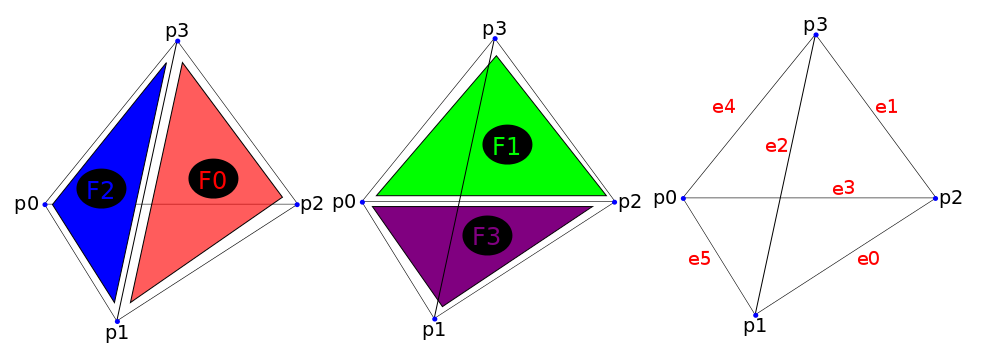
\includegraphics[width=1.0\linewidth]{figures/cutting/tetconfig3.png}
  \caption{\label{fig:tetconfig3}
  {A tetrahedral element in its canonical view. Iterating over nodes, edges and faces of each element is
  one of the primary operations in a geometric algorithm that manipulates such elements.}
}
\end{figure}

%Most of these challenges are due to the contradictory requirements of speed versus the fidelity of the cutting surfaces. 
%%In our experience the following major points required extra effort and validation:

